\section{Experiment 5: colour, inversion and reversal}

\subsection{Methodology}


\paragraph{Stimuli}

A 1000-frame corpus of consecutive fire images was used.



\paragraph{Subjects}

10 subjects were recruited using a mailing list operated by University College London. All reported normal or corrected-to-normal vision.

\paragraph{Trial structure}

Delayed match-to-sample with altered sample.
In each trial, a sample was presented first, followed by two tests. A manipulation was applied to the sample; the tests were unchanged. Subjects indicated which test they thought corresponded to the sample using the left arrow (first sample) and right arrow (second sample) keys. 

Sample length (sL) was 50 frames (1 second)
Test length was 60 frames (1.2 seconds)

\paragraph{Factors}

We varied the manipulation applied to the sample clips:
none, luminance-inverted,colour-inverted, backwards, or spatially inverted.

\paragraph{Block structure}

Firstly, we presented 24 training trials

Next, we presented 30 training trials with dynamic samples and tests and the same clip lengths, but with samples and tests unaltered.

We presented 5 blocks (corresponding to each manipulation) in random order.

We used 80 trials per block, a total of  400 trials.


\begin{figure}[H]
\centering
\renewcommand{\arraystretch}{1.8}

      \begin{subfigure}[b]{\textwidth}
\begin{tabular}{ >{\bfseries}r | p{8cm}   }
& \textbf{Experiment 3}\\
\hline
  
Design & 2AFC delayed match-to-sample, with filtered or inverted sample\\                   
Stimuli & 1000-frame corpus\newline
		1 second sample (50 frames)\newline
		1.2 second test (60 frames)\\
Factors & Manipulation:\newline
		a) none\newline
		b) colour inversion\newline
		c) luminance inversion\newline
		d) temporal inversion\newline
		e) spatial inversion\\

Block design & Manipulation varied across blocks\newline
		5 blocks in random order\newline
80 trials per condition \newline
400 trials \\
Training &25 training trials \\
Subjects&10\\
\end{tabular}
\caption{Design summary.}
   \end{subfigure}

\begin{subfigure}[b]{\textwidth}
\centering
                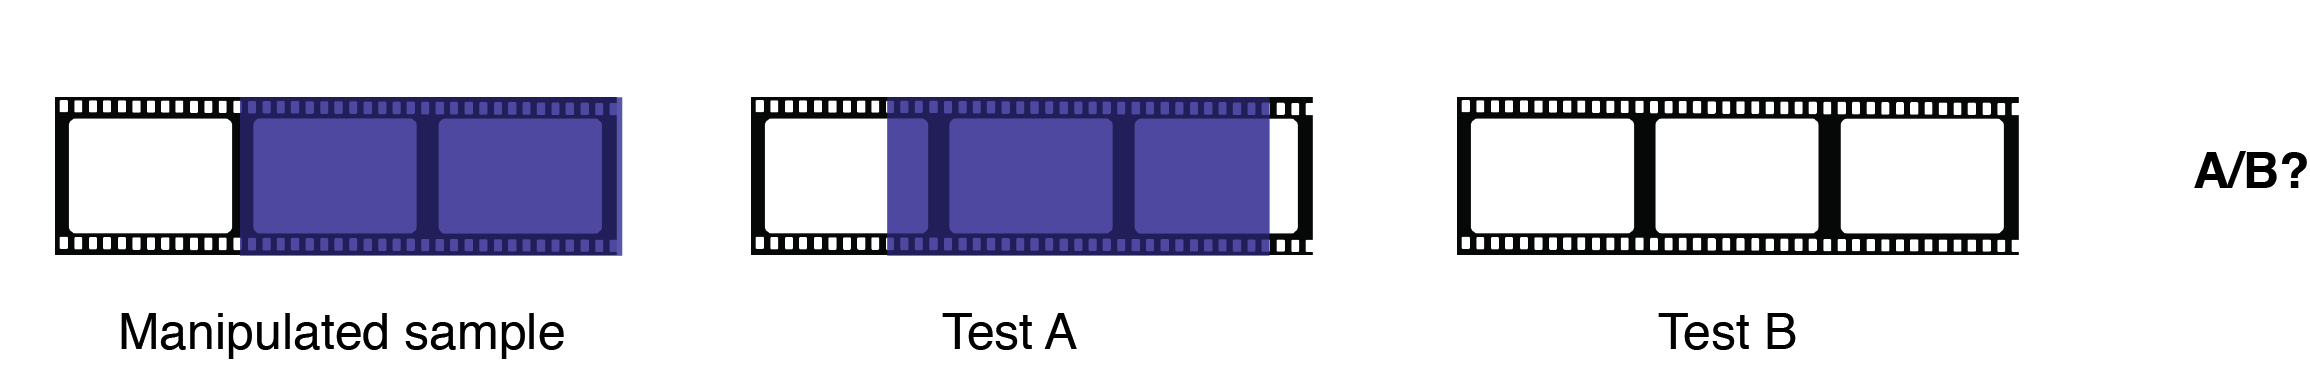
\includegraphics[width=12cm]{img/fire5protocol.png}
                \caption{An altered (filtered or inverted) sample was followed by two untouched tests, one of which contained the sample.}     
        \end{subfigure}
\caption{Experiment 4: design summary and trial structure.}
\end{figure}

\begin{figure}[htp]
\centering
\begin{subfigure}[b]{0.5\textwidth}
\centering
                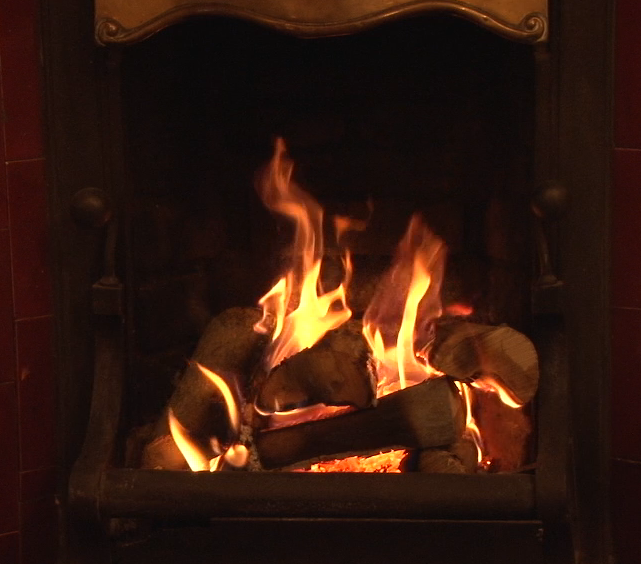
\includegraphics[width=5cm]{img/frame00003.png}
                \caption{Normal}         
        \end{subfigure}\begin{subfigure}[b]{0.5\textwidth}
\centering
                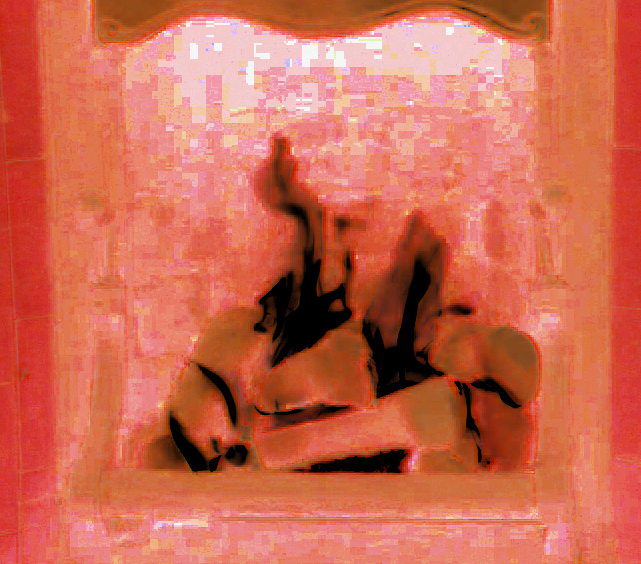
\includegraphics[width=5cm]{img/frame00001.png}
                \caption{Luminance inverted}         
        \end{subfigure}

\begin{subfigure}[b]{0.5\textwidth}
\centering
                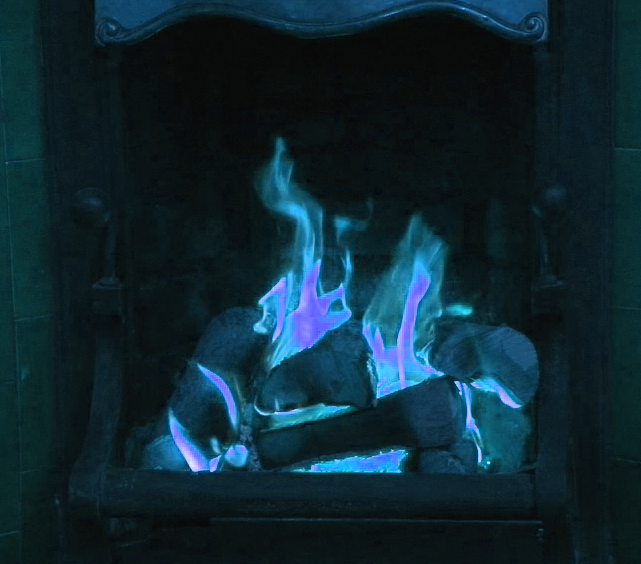
\includegraphics[width=5cm]{img/frame00002.png}
                \caption{Hue inverted}         
        \end{subfigure}\begin{subfigure}[b]{0.5\textwidth}
\centering
                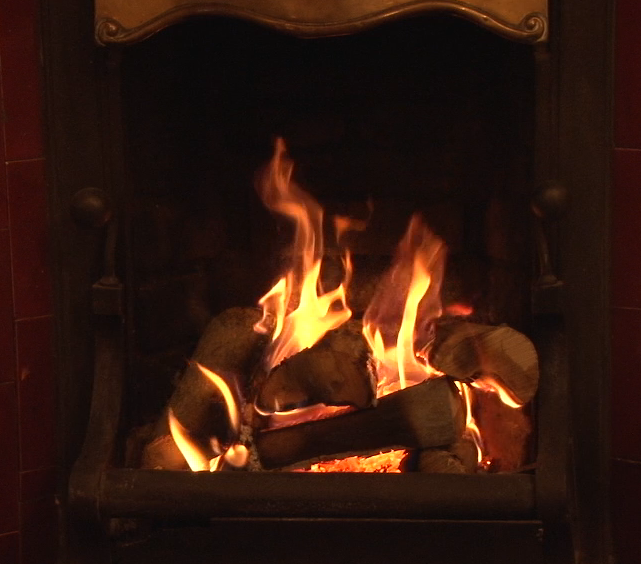
\includegraphics[width=5cm,angle=180]{img/frame00003.png}
                \caption{Spatially inverted}         
        \end{subfigure}

\caption{Experiment 4: Examples of the manipulations we used, applied to one frame. Reversal is not shown.}
\end{figure}

\subsection{Results}

\paragraph{Accuracy by manipulation}

We observed the following mean accuracies:

\begin{center}
\begin{tabular}{ r | l   }
\textbf{Sample manipulation} & \textbf{Mean accuracy}\\
\hline
None&  0.60\\
Negative&  0.59\\
Chromatic& 0.61\\
Reversed&  0.58\\
Inverted&  0.59\\
\end{tabular}
\end{center}

Single-sample $t$-tests showed that subjects were more accurate than chance ($p$<0.05) under each one of these conditions. However, paired-samples $t$-tests showed no difference in means between any pair of conditions ($p$>0.2 in each case).

\paragraph{Learning}

\begin{figure}[htp]
\centering
\begin{subfigure}[b]{\textwidth}
\centering
                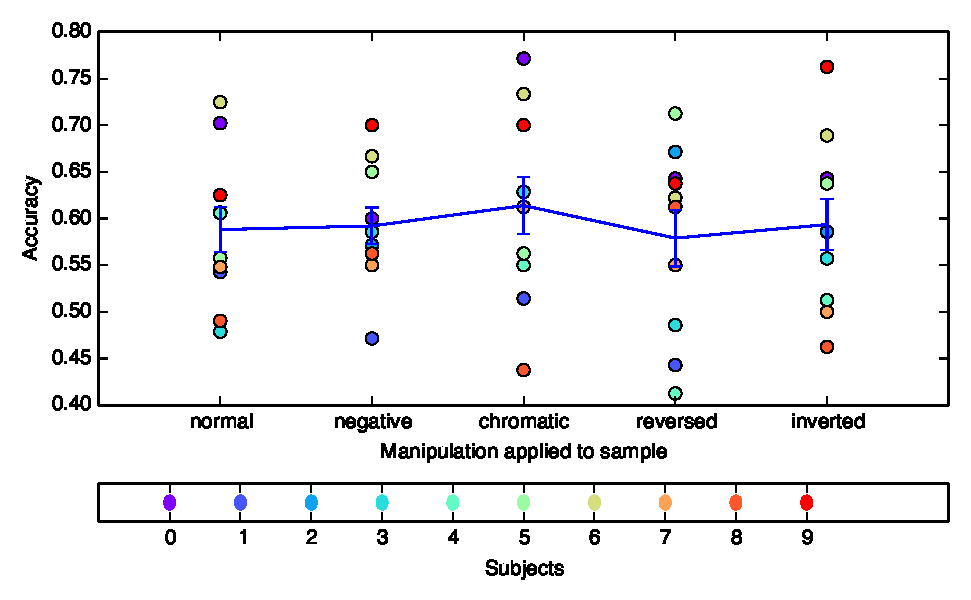
\includegraphics[width=12cm]{img/fig_fire5-manips1_correct_manip.pdf}
                \caption{Accuracy in function of the five manipulations.}
          
        \end{subfigure}

\caption{Experiment 3: Detection was above chance under all manipulations, but was too low to discern a contrast between the effects.}
\end{figure}

\subsection{Discussion}